\documentclass[11pt]{article}
\usepackage[margin=1in]{geometry}
\usepackage[T1]{fontenc}
\usepackage{lmodern}
\usepackage{microtype}
\usepackage{amsmath}
\usepackage{booktabs}
\usepackage{graphicx}
\usepackage{caption}
\usepackage[hidelinks]{hyperref}
\graphicspath{{figures/}}
\captionsetup{font=small,labelfont=bf}
\setlength{\parskip}{0.4em}

\title{\textbf{Adaptive Chunk-Based Compression\\for Inverted Index Posting Lists}}
\author{Cooper Malone\\University of Nebraska--Lincoln}
\date{}

\begin{document}
\maketitle

\begin{abstract}
\noindent
Search engines compress the integer lists in their inverted indexes, usually with a single codec
for the whole index. Real posting lists are not uniform: dense runs of small gaps sit next to sparse
stretches of large ones, and different codecs suit each. This project implements three classic
integer codecs (variable-byte, Elias gamma and bit packing) and an adaptive scheme that splits each
list into fixed-size chunks, encodes every chunk with all three codecs, and keeps the smallest result
together with a one-byte codec identifier. On synthetic lists that mix several gap patterns, the
adaptive scheme is 49\% smaller than the best single codec applied to the whole list and 29\%
smaller than the best single codec applied chunk by chunk. On lists with one consistent pattern it
is never best, but it stays within 2\% of the best codec applied to the same chunks, without knowing
that codec in advance. On a positional
index of Shakespeare's complete works, however, vByte wins 98\% of chunks, and the identifiers cost
more than adaptivity saves: the adaptive index is 3--4\% larger than plain vByte. Encoding the
identifiers with an entropy code would reverse this, for an estimated 0.2--0.6\% gain. Adaptive
compression is therefore worth its cost when lists are long and heterogeneous, and the decision
overhead must be kept far below one byte per chunk when most lists are short.
\end{abstract}

\section{Introduction}

An inverted index maps each term to a \emph{posting list}, the sorted document identifiers or word
positions at which the term occurs. Because the lists are sorted, they are stored as \emph{gaps}
(differences between consecutive entries), which are mostly small integers, and the gaps are
compressed with an integer codec~\cite{manning2008}. A smaller index needs less memory and disk
bandwidth, so the choice of codec affects both storage cost and query speed.

Most systems choose one codec for every list. That choice assumes the gaps follow one distribution
throughout the index, but they do not: a frequent term has long lists of tiny gaps, a rare term has
a few large gaps, and a single list can alternate between dense and sparse regions. A codec that is
efficient in one region can be wasteful in another.

This project asks whether choosing the codec locally, chunk by chunk, makes an index smaller, and
what that choice costs. Its contributions are:
\begin{itemize}
  \item from-scratch implementations of variable-byte (vByte), Elias gamma and bit-packing codecs,
        with a 98-test suite that checks every codec round-trips correctly;
  \item an adaptive chunked compressor that selects the smallest codec for each chunk and records its
        choice;
  \item a benchmark on synthetic gap patterns and on a real positional index that separates the
        benefit of chunking from the benefit of choosing a codec, and that charges the adaptive scheme
        for the identifiers it stores.
\end{itemize}

\section{Background and Related Work}

\textbf{Variable-byte (vByte)} coding stores an integer in 7-bit groups, one group per byte, and uses
the remaining bit of each byte to mark whether another byte follows. It is byte-aligned and fast to
decode, but it spends at least 8 bits on every integer, even a gap of 1.

\textbf{Elias gamma} coding~\cite{elias1975} writes a positive integer $x$ as $\lfloor\log_2 x\rfloor$
zeros followed by the binary form of $x$, for $2\lfloor\log_2 x\rfloor + 1$ bits in total. It is
excellent for very small values and poor for large ones, and because it is bit-aligned it is slower
to decode.

\textbf{Bit packing}, often called frame of reference, stores a block of integers at one fixed bit
width, the width needed for the largest value in the block after subtracting the block minimum. It
is compact when the values in a block are similar and wasteful when one outlier forces a wide width
on every value.

Block-based codecs are standard in practice. Simple-9 packs as many small integers as fit into a
32-bit word~\cite{anh2005}, PForDelta bit-packs a block and stores the few outliers
separately~\cite{zukowski2006}, and vectorized variants decode billions of integers per
second~\cite{lemire2015}. The idea closest to this project is partitioned Elias--Fano
coding~\cite{ottaviano2014}, which splits each list into variable-length partitions and encodes each
one with whichever representation is smallest. The present project studies a simpler version of
that idea: fixed-size chunks and a choice among three general-purpose codecs.

\section{Methods}

\subsection{Codecs}

All three codecs encode a sequence of non-negative integers. When they compress a posting list,
the first position in each chunk is stored as is and each later position is stored as its gap
from the previous one.
\begin{itemize}
  \item \textbf{vByte} encodes an integer $x$ in $\max(1,\lceil b(x)/7\rceil)$ bytes, where $b(x)$ is
        the number of bits in $x$.
  \item \textbf{Elias gamma} encodes $x+1$ (so that zero can be represented), using
        $2\lfloor\log_2(x+1)\rfloor+1$ bits. A buffered bit writer lets codes cross byte boundaries,
        and the final byte is padded.
  \item \textbf{Bit packing} writes a 9-byte header (the minimum value, the bit width $w$ and the
        count $n$) followed by $\lceil nw/8\rceil$ bytes of packed values, where
        $w = b(\max - \min)$.
\end{itemize}

\subsection{Chunking}

A list of length $n$ is split into $\lceil n/k\rceil$ consecutive chunks of $k$ integers (the last
may be shorter), and each chunk is compressed independently. Chunking lets a decoder skip to the
chunk it needs, and it lets bit packing use a narrower width when values are similar within a chunk
even though they vary across the list.

\subsection{Adaptive selection}

The adaptive compressor encodes each chunk with every codec, keeps the shortest output and prepends
a one-byte codec identifier. Decoding reads the identifier and calls that codec's decoder, so
decompression costs the same as with a single codec. Compression costs roughly the sum of the three
codecs' encoding times, because every chunk is encoded three times. By construction the adaptive
output for a list is never larger than the best \emph{chunked} single codec plus one byte per chunk.

\section{Experimental Setup}

\subsection{Data}

\textbf{Synthetic lists.} Each list holds 10{,}000 integers drawn with a fixed random seed:
\begin{itemize}
  \item \emph{Uniform, small values}: uniform on $\{0,\dots,10\}$;
  \item \emph{Clustered}: $1000 + U\{0,\dots,5\}$, large values that vary little;
  \item \emph{Sparse with outliers}: 95\% uniform on $\{1,\dots,5\}$ and 5\% uniform on
        $\{1000,\dots,100000\}$;
  \item \emph{Increasing positions}: running sums of gaps uniform on $\{1,\dots,5\}$, compressed
        without gap encoding, so the values grow steadily to about 30{,}000;
  \item \emph{Mixed}: the four patterns above alternating in blocks of 1{,}000 values within one
        list, the setting that motivates choosing a codec per chunk.
\end{itemize}

\textbf{Real text.} The complete works of Shakespeare (\texttt{t8.shakespeare.txt}, the Project
Gutenberg edition) were tokenized on whitespace and lowercased, giving 901{,}325 tokens and 59{,}508
distinct terms. Each term's posting list holds the word positions at which it occurs, so the index
is a positional index of one long document. Half of the terms (31{,}079, or 52\%) occur exactly
once. Uncompressed, at 4 bytes per position, the index occupies 3{,}605{,}300 bytes. An earlier
run on a 1{,}928-document subset of the 20 Newsgroups collection showed the same ordering of vByte
and Elias gamma (compression ratios 0.363 and 0.477), but that subset could not be re-run with the
identifier accounting below, so it is not reported further.

\subsection{Metrics and procedure}

For the synthetic lists the measure is compressed size in bytes. Each codec is applied once to the
whole list, and once chunk by chunk with $k = 128$; the adaptive scheme uses the same chunks. For
the real index the measure is the \emph{compression ratio}, compressed size divided by
uncompressed size (lower is better), at chunk sizes $k \in \{50, 100, 200, 500\}$. The adaptive
scheme is charged one byte per chunk for its identifier; Section~\ref{sec:real} also reports it with
no identifier cost and with an ideal 2-bit identifier. Compression time is the wall-clock time to
encode the whole index, averaged over the four chunk sizes and three repetitions, using single-threaded
Python 3.12 on an AMD Ryzen 7 7800X3D. Every compressed list was decoded and checked against the
original. All numbers in this report are produced by \texttt{report/make\_figures.py}.

\section{Results}

\subsection{Synthetic lists}

Table~\ref{tab:synthetic} and Figure~\ref{fig:synthetic} show the compressed sizes. No single codec
wins every pattern. Bit packing is best on uniform and clustered values, where a narrow fixed width
fits every value, but it is the worst codec on sparse data, because a single outlier near 100{,}000
forces 17 bits onto all 10{,}000 values. Elias gamma is best on sparse data with outliers and worst
on clustered values near 1{,}000. vByte is never best: it spends at least one byte on every value.

\begin{table}[h]
\centering
\small
\begin{tabular}{lrrrrr}
\toprule
 & \multicolumn{3}{c}{Whole list} & \multicolumn{1}{c}{Best codec,} & \\
\cmidrule(lr){2-4}
Dataset & vByte & Elias $\gamma$ & Bit pack & \multicolumn{1}{c}{chunked} & Adaptive \\
\midrule
Uniform, small values & 10{,}000 & 6{,}238 & \textbf{5{,}009} & 5{,}711 (bit pack) & 5{,}781 \\
Clustered             & 20{,}000 & 23{,}750 & \textbf{3{,}759} & 4{,}461 (bit pack) & 4{,}540 \\
Sparse with outliers  & 10{,}978 & \textbf{6{,}982} & 21{,}259 & 7{,}012 (Elias $\gamma$) & 7{,}091 \\
Increasing positions  & 24{,}452 & 33{,}509 & 18{,}759 & \textbf{11{,}955} (bit pack) & 12{,}034 \\
Mixed                 & 15{,}083 & 15{,}415 & 21{,}259 & 10{,}749 (bit pack) & \textbf{7{,}647} \\
\bottomrule
\end{tabular}
\caption{Compressed size in bytes of 10{,}000-integer synthetic lists (lower is better). Chunked
results use chunks of 128 integers; the adaptive size includes 79 one-byte codec identifiers. The
smallest size in each row is in bold.}
\label{tab:synthetic}
\end{table}

\begin{figure}[h]
\centering
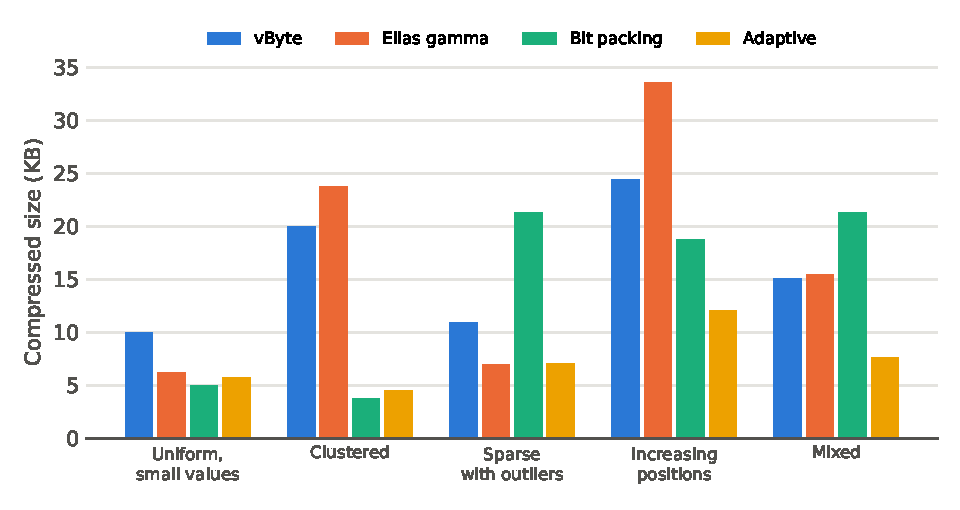
\includegraphics[width=0.82\textwidth]{synthetic_sizes.pdf}
\caption{Compressed size of each synthetic list. vByte, Elias gamma and bit packing are applied to
the whole list; adaptive chooses a codec for each 128-integer chunk.}
\label{fig:synthetic}
\end{figure}

The chunked column separates two effects. On \emph{increasing positions}, adaptive is 36\% smaller
than the best whole-list codec, but nearly all of that comes from chunking: bit packing each chunk
on its own subtracts a local minimum, and that alone reaches 11{,}955 bytes. Chunking can also hurt:
on uniform and clustered values, repeating bit packing's 9-byte header in every chunk makes the
chunked result 14--19\% larger than packing the whole list at once. Wherever one codec suits the
whole list, the adaptive scheme ends up 0.7--1.8\% larger than the best codec applied to the same
chunks, roughly the cost of its 79 identifiers. The \emph{mixed} list is different. No single codec suits
every block, and choosing per chunk makes the adaptive output 29\% smaller than the best chunked
single codec and 49\% smaller than the best whole-list codec. This is the case adaptive compression
is designed for, and here it clearly pays off.

\subsection{Real text}
\label{sec:real}

On the Shakespeare index (Table~\ref{tab:real}, Figure~\ref{fig:real}), vByte compresses best among
the single codecs at every chunk size, to about 45\% of the original size. Elias gamma reaches about
59\%, and bit packing 69--75\%, because its 9-byte header is large compared with the many lists
that contain only a few positions.

\begin{table}[h]
\centering
\small
\begin{tabular}{rrrrrrrr}
\toprule
 & & & & & \multicolumn{3}{c}{Adaptive, identifier cost} \\
\cmidrule(lr){6-8}
Chunk size & Chunks & vByte & Elias $\gamma$ & Bit pack & none & 2 bits & 1 byte \\
\midrule
50  & 72{,}319 & \textbf{0.4566} & 0.5998 & 0.7508 & 0.4557 & 0.4607 & 0.4757 \\
100 & 65{,}328 & \textbf{0.4539} & 0.5939 & 0.7269 & 0.4523 & 0.4569 & 0.4705 \\
200 & 62{,}113 & \textbf{0.4526} & 0.5910 & 0.7106 & 0.4504 & 0.4547 & 0.4676 \\
500 & 60{,}388 & \textbf{0.4518} & 0.5895 & 0.6935 & 0.4487 & 0.4529 & 0.4655 \\
\bottomrule
\end{tabular}
\caption{Compression ratio (compressed / original size, lower is better) on the positional index of
Shakespeare. The adaptive scheme is shown with no identifier cost, with an ideal 2-bit identifier and
with the 1-byte identifier it actually stores. The best realizable result in each row is in bold.}
\label{tab:real}
\end{table}

\begin{figure}[h]
\centering
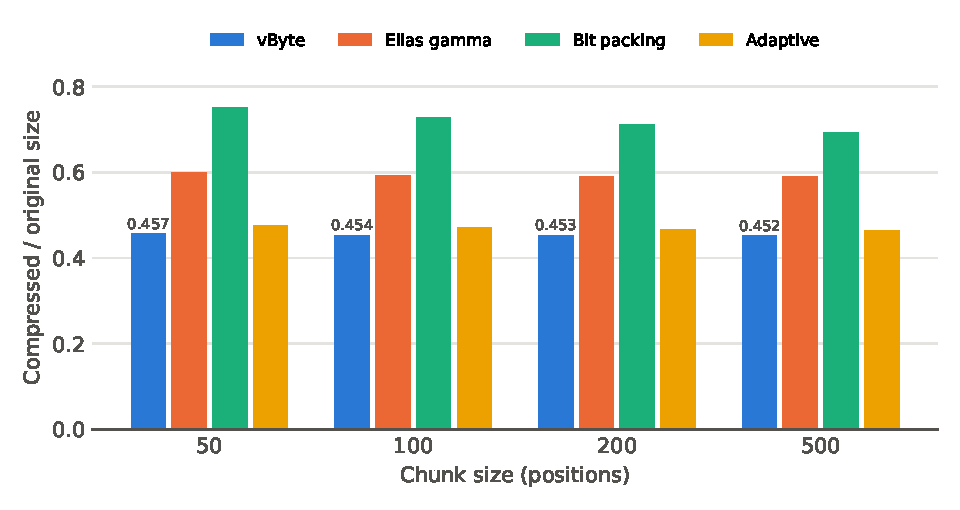
\includegraphics[width=0.82\textwidth]{real_text_ratio.pdf}
\caption{Compression ratio on the Shakespeare positional index by chunk size. The adaptive bars
include its 1-byte codec identifiers.}
\label{fig:real}
\end{figure}

The adaptive scheme picks vByte for 97.8--98.5\% of chunks, bit packing for 1.4--2.2\% and Elias gamma
for fewer than 0.1\%. If its choices were free, it would beat vByte by 3{,}560 to 11{,}125 bytes, or
0.1--0.3 percentage points of compression ratio. But the index has more than 60{,}000 chunks, at least one
per term, and storing one byte per chunk costs 60--72~KB, 5 to 20 times what adaptivity saves. Even an
ideal 2-bit identifier costs 15--18~KB, still more than the saving. With identifiers counted, the
adaptive index is 3.0--4.2\% larger than plain vByte.

\subsection{Compression time}

Adaptive compression is the slowest, as expected (Figure~\ref{fig:time}). Encoding the full index took
0.31~s with vByte, 0.33~s with bit packing, 1.17~s with Elias gamma and 1.81~s with the adaptive
scheme, 5.8 times as long as vByte. These are pure-Python timings, so their ratios are more
meaningful than their absolute values. Decompression needs a single decoder per chunk and is not
slowed by adaptivity.

\begin{figure}[h]
\centering
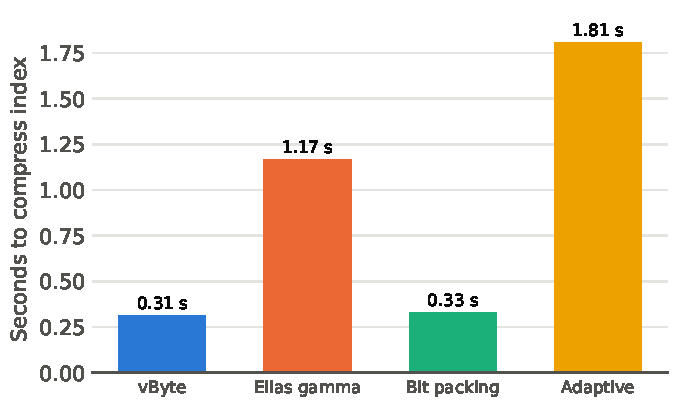
\includegraphics[width=0.55\textwidth]{compression_time.pdf}
\caption{Mean time to compress the full Shakespeare index (four chunk sizes, three repetitions each).}
\label{fig:time}
\end{figure}

\section{Discussion}

The results answer the project's question in two parts. First, choosing a codec per chunk is
valuable exactly when the data inside a list are heterogeneous. On the mixed list it removed almost
half of the best fixed codec's output. On homogeneous lists it cannot beat the best codec at the same
chunk size, but it comes within 2\% of it without having to know in advance which codec that is. This makes it a robust
default when the data are unknown.

Second, the cost of the decision matters as much as its benefit. A natural-language index is
dominated by short lists: half of Shakespeare's terms occur once, so most chunks are tiny and a byte
spent on an identifier is large compared with the data it describes. For such an index the decision
must be made far more cheaply. One way is to entropy-code the identifiers. The choices are very
skewed (about 98\% vByte), with an entropy of only 0.12--0.15 bits per chunk, so an ideal
entropy code would cost about 1.1~KB in total. The adaptive index would then beat vByte by
2.5--10.0~KB, or 0.15--0.61\%. This estimate ignores the small cost of storing the code itself, but
it shows that the idea can win on real text once its overhead is controlled. Other remedies are to
apply adaptivity only to lists longer than one chunk, or to choose the partitions as well as the
codecs, as partitioned Elias--Fano does~\cite{ottaviano2014}.

\paragraph{Limitations.} The implementation is in pure Python, so the timings show relative cost,
not the speed of a production codec. The real-text evaluation uses one corpus and a positional index
of a single document; a document-level index of a web collection would have a different mix of
list lengths. The synthetic patterns, including the mixed list, were designed for this study and do
not show how often such heterogeneity occurs in real indexes.

\section{Conclusion and Future Work}

Adaptive chunk-based compression chose well: it was never more than 2\% worse than the best single
codec at the same chunk size, and it was far better when a list mixed patterns. On a real index of short lists,
though, storing its decisions costs more than the decisions save, and plain vByte remains the better
choice unless the identifiers are compressed. Promising next steps are
\begin{itemize}
  \item entropy-coding the codec identifiers, or sharing one identifier across a whole short list;
  \item choosing chunk boundaries adaptively instead of using a fixed chunk size;
  \item replacing exhaustive trial encoding with a cheap predictor of the best codec, based on the
        mean, variance and maximum gap of a chunk, to cut compression time;
  \item evaluating on large document-level indexes such as web or news collections.
\end{itemize}

\begin{thebibliography}{9}
\small
\bibitem{anh2005} V.~N.~Anh and A.~Moffat. Inverted index compressed using word-aligned binary
codes. \emph{Information Retrieval}, 8(1):151--166, 2005.

\bibitem{elias1975} P.~Elias. Universal codeword sets and representations of the integers.
\emph{IEEE Transactions on Information Theory}, 21(2):194--203, 1975.

\bibitem{lemire2015} D.~Lemire and L.~Boytsov. Decoding billions of integers per second through
vectorization. \emph{Software: Practice and Experience}, 45(1):1--29, 2015.

\bibitem{manning2008} C.~D.~Manning, P.~Raghavan and H.~Sch\"utze. \emph{Introduction to
Information Retrieval}, Chapter~5. Cambridge University Press, 2008.

\bibitem{ottaviano2014} G.~Ottaviano and R.~Venturini. Partitioned Elias--Fano indexes. In
\emph{Proceedings of the 37th International ACM SIGIR Conference}, pages 273--282, 2014.

\bibitem{zukowski2006} M.~Zukowski, S.~H\'eman, N.~Nes and P.~Boncz. Super-scalar RAM-CPU cache
compression. In \emph{Proceedings of the 22nd International Conference on Data Engineering (ICDE)},
2006.
\end{thebibliography}

\end{document}
